%----------------------------------------------------------------------------------------
%	Introducción
%----------------------------------------------------------------------------------------

\newpage
\clearpage{\pagestyle{empty}\cleardoublepage}
%\doublespacing
\newpage

\chapter*{\centering \large Introducción} 
\addcontentsline{toc}{chapter}{Introducción} % si queremos que aparezca en el índice
\markboth{Introduction}{Introducción} % encabezado

Según FAO (\textit{Food and Agriculture Organization of the United Nations}), el salmón y la trucha fueron los productos de pesquería más comercializados en términos de valor desde 2013 y representan alrededor de 18\% del valor total de los productos pesqueros comercializados internacionalmente desde 2017. \cite{FAO2017} La producción de truchas, en lagunas y ríos en los andes, es responsable de un cuarto de la producción acuícola en el Perú.\cite{SeafoodTradeIntelligencePortal2018} Sin embargo, según FONDEPES (\textit{Fondo Nacional de Desarrollo Pesquero}), la región Puno centraliza dicha producción con el 82.1\% en el 2017 de la producción nacional de truchas con más de 18000 TM/Año y un porcentaje de esta se da artesanalmente.\cite{FONDEPES2014} Perú ha incrementado 348.3\% la extracción de truchas en los últimos 10 años.\cite{MinisteriodelaProducciondelPeru2018}

Sin embargo, Perú cuenta con lagos y lagunas que son potenciales lugares de crianza de truchas que no son explotados debido a que se requiere un esfuerzo alto en mano de obra. Además, el costo de automatización con máquinas comerciales importadas es alto y no está destinado a pequeñas y medianas empresas. Entonces, este \textbf{trabajo de investigación} realiza un pequeño aporte a la automatización de la industria pesquera nacional. Específicamente en dos procesos que se dan cada cierto período de tiempo a medida que las truchas van aumentando sus dimensiones: la clasificación por tallas y conteo de truchas. El trabajo de investigación consta de tres capítulos: \textbf{marco problemático}, \textbf{diseño mecatrónico conceptual} y \textbf{conclusiones}.

%\vspace{1.5cm}
%\begin{figure}[H]
%\centering
%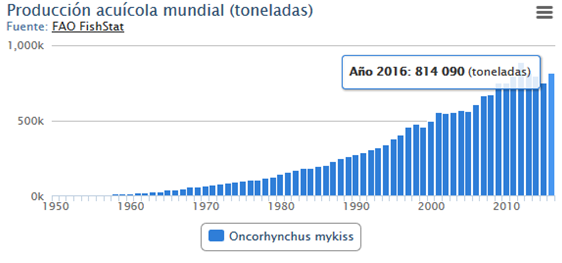
\includegraphics[width=1\textwidth]{introduction/produccion agricola mundial.png}
%\caption{Ejemplo de imagen.}
%\label{fig:PLACEHOLDER}
%\end{figure}